\documentclass[a4paper, 14pt, oneside]{Thesis}
\usepackage{ulem}
\usepackage[square, numbers, comma, sort&compress]{natbib}  % Use the "Natbib" style for the references in the Bibliography
\usepackage{verbatim} 
\usepackage{pslatex} %To set the font as Times New Roman
\usepackage{amsbsy} 
\usepackage{amsfonts}
\usepackage{graphicx}
\usepackage{dcolumn}
\usepackage{amsmath}
\usepackage{latexsym}
\usepackage{amssymb}
\usepackage{epsfig}
\usepackage{verbatim} 
\usepackage{epsfig,graphics}
\usepackage{amsmath, amsthm, amssymb}
\usepackage{subfigure}
\usepackage{tikz}
\usepackage{adjustbox}
\usepackage{glossaries}
\usepackage{csquotes}
%\usepackage{fancyhdr}
%\usepackage{lipsum}

%To have 1. instead of [1] in the bibliographic entry
\makeatletter
\renewcommand\@biblabel[1]{#1.}
\makeatother

% To remove hyphenation
\tolerance=1
\emergencystretch=\maxdimen
\hyphenpenalty=10000
\hbadness=10000
%
%----To make sure the page numbers are in the top middle of each page.
\fancypagestyle{Thesis}{
\fancyhf{}
\fancyhead[C]{\thepage}
%\lfoot{\thepage}
\cfoot{\thepage}
\pagestyle{fancy}
}
%redefine the plain pagestyle
%\fancypagestyle{plain}{
%\fancyhf{}
%\fancyhead[C]{\thepage}
%}
%----------------------------------------------------------------------
%% ------------------------s----------------------------------------
% Some new environments for the paper
%
\newtheorem{dfn}{Definition}[section]
\newtheorem{prop}[dfn]{Proposition}
\newtheorem{lem}[dfn]{Lemma}
\newtheorem{thm}[dfn]{Theorem}
\newtheorem{cor}[dfn]{Corollary}
\newtheorem{clm}[dfn]{Claim}
\newtheorem{fact}[dfn]{Fact}
%
%\newcommand{\RightBox}{\begin{flushright} $\Box$ \end{flushright}}
\newcommand{\RightBox}{{\phantom{a}}\hfill $\Box$ \\}
%\newenvironment{proof}{{\bf Proof:~}}{\RightBox}
\newenvironment{prf}{{\bf Proof~Idea:~}}{\RightBox}
%\newcommand{\claim}[1]{{\bf Claim #1:~}}
%
\newcommand{\Dfn}[1]{Definition \ref{dfn:#1}}
\newcommand{\Prop}[1]{Proposition \ref{prop:#1}}
\newcommand{\Lem}[1]{Lemma \ref{lem:#1}}
\newcommand{\Thm}[1]{Theorem \ref{thm:#1}}
\newcommand{\Cor}[1]{Corollary \ref{cor:#1}}

%Action-indexed diamond modality
\newcommand{\Adiam}[1]{\mbox{$\langle #1 \rangle$}}
\newcommand{\diamin}{\Diamond\kern-0.5em{\raisebox{.25ex}{\rm -}}\kern0.175em}
\newcommand{\until}{\mbox{\large\bf U}}
\newcommand{\since}{\mbox{\large\bf S}}
\newcommand{\nxt}{\mbox{$\bigcirc$}}
\newcommand{\nxtdot}{\displaystyle \bigodot}
\newcommand{\past}{\diamin}
\newcommand{\ifpast}{\mbox{$\boxminus$}}
\newcommand{\now}{\mbox{$\langle now \rangle$}}
\newcommand{\Now}{\mbox{$[now]$}}
\newcommand{\pres}{\mbox{$\rangle \langle$}}
\newcommand{\snd}{\mbox{\large\bf s}}
\newcommand{\rec}{\mbox{\large\bf r}}
\newcommand{\nc}{\mathbf{no\_comm}}

%Propositional connectives
%\newcommand{\implies}{{\raisebox{.20ex}{$\scriptstyle ~\supset~$}}}
\newcommand{\Not}{\mbox{$\lnot$}}
\newcommand{\xor}{\oplus}
\newcommand{\True}{\mathit{True}}
\newcommand{\False}{\mathit{False}}
\newcommand{\Imply}{\supset}
%Large symbols
\newcommand{\andover}{\displaystyle \bigwedge}
\newcommand{\orover}{\displaystyle \bigvee}
\newcommand{\capover}{\displaystyle \bigcap}
\newcommand{\cupover}{\displaystyle \bigcup}
\newcommand{\piover}{\displaystyle \Pi}
\newcommand{\ohat}[1]{\widehat{#1}}
\newcommand{\otilde}[1]{\widetilde{#1}}
\newcommand{\obar}[1]{\overline{#1}}
\newcommand{\Sigtil}{\mbox{$\otilde{\Sigma}$}}
\newcommand{\DA}{\mbox{$\Sigtil~=~(\Sigma_1, \dots, \Sigma_n)$}}

%Useful symbols
\newcommand{\derives}{\vdash}
\newcommand{\defn}{\mbox{$~\stackrel{\rm def}{=}~$}}
\newcommand{\qneq}{\mbox{$~\stackrel{\rm ?}{=}~$}}
\newcommand{\eqv}{\approx}
\newcommand{\hash}{\sharp}
\newcommand{\restr}{\lceil}
%\newcommand{\bot}{\bottom}
\newcommand{\nat}{{\bf N}}
\newcommand{\pfin}[1]{\mbox{$\wp_{fin}(#1)$}}
%\newcommand{\mod}[1]{\mbox{$|#1|$}}
\newcommand{\memb}[2]{\mbox{${#1} \in {#2}$}}
\newcommand{\E}{\mathbf{E}}



%Some roman words in math mode
\newcommand{\Iff}{\mbox{~iff~}}
\newcommand{\For}{\mbox{~for~}}
\newcommand{\Where}{\mbox{~where~}}
%\newcommand{\And}{\mbox{~and~}}
\newcommand{\Implies}{\mbox{~implies~}}

%Relations

% structures
\newcommand{\Sigstr}{\mbox{$\Sigma^*$}}
\newcommand{\TS}{\mbox{$TS = (Q,\to)$}}  %generates TS=(Q,->)
\newcommand{\TSP}{\mbox{$TS = (Q,\To)$}}         %generates TS=(Q,=>)
\newcommand{\TSi}{\mbox{$TS_i = (Q_i,\to_i)$}}           
\newcommand{\TSE}{\mbox{$TS_{ES}$}}
\newcommand{\TSN}{\mbox{$TS_{\cal N}$}}
\newcommand{\ES}{\mbox{$ES = (E,\leq,\#)$}}       %generates ES=(E,<=,#)
\newcommand{\LES}{\mbox{$ES = (E,\leq,\#,\phi)$}} %generates ES=(E,<=,#,phi)
\newcommand{\Tmdl}{\mbox{$M = (TS,V)$}}          %generates M = (TS,V)
\newcommand{\cfin}[1]{\mbox{$C_{#1}$}}           %finite configurations of
\newcommand{\fincon}[1]{\mbox{$C_{#1}^{fin}$}}  %finite configurations

% classes
\newcommand{\mdl}[1]{\mbox{${\cal M}_{#1}$}}%generates script M with subscript
\newcommand{\dmodels}{\mbox{$\models_{Det}~$}}

% For transitions steps
\newcommand{\step}[1]{\mbox{$\stackrel{#1}{\to}$}}
\newcommand{\Funnyto}{\rightsquigarrow}
\newcommand{\longstep}[1]{\mbox{$\stackrel{#1}{\longrightarrow}$}}
\newcommand{\emptystep}{\step{\emptyset}}
\newcommand{\reach}[1]{\mbox{${\cal R}(#1)$}}
\newcommand{\reachin}[2]{\mbox{${\cal R}_{#1}(#2)$}}

% For a "double-lined" transition relation
\newcommand{\To}{\Rightarrow}
\newcommand{\From}{\Leftarrow}
\newcommand{\Step}[1]{\mbox{$\stackrel{#1}{\To}$}}
\newcommand{\Longstep}[1]{\mbox{$\stackrel{#1}{\Longrightarrow}$}}
\newcommand{\Longlongstep}[1]{\mbox{$\stackrel{#1}{\Longlongrightarrow}$}}
\newcommand{\Emptystep}{\Step{\emptyset}}

% Net theory
\newcommand{\presca}[1]{\mbox{${ }^{\bullet}#1$}}
\newcommand{\postsca}[1]{\mbox{$#1 \, { }^{\bullet}$}}%

%The built in downarrow generates too much space after it
%\newcommand{\down}{\mbox{$\downarrow \!$}}
\newcommand{\down}{\mbox{$\downarrow$}}
\newcommand{\up}{\mbox{$\uparrow \!$}}
\newcommand{\ldot}{{\rm <}\kern-0.37em{\raisebox{.25ex}{\bf .}}\kern0.375em}

%Trace theory
\newcommand{\edoti}{\mbox{$\doteq_I$}}
\newcommand{\eqi}{\mbox{$=_I$}}
\newcommand{\edotk}{\mbox{$\doteq_k$}}
\newcommand{\eqk}{\mbox{$=_k$}}

\newcommand{\calL}{\mathcal{L}}
\newcommand{\calB}{\mathcal{B}}
\newcommand{\posetlang}[1]{\mbox{${\calL}^{po}(#1)$}}%poset language of an SCA
\newcommand{\bddlang}[2]{\mbox{${{\calL}^{#1}}(#2)$}} %bounded buffer language

\newcommand{\calS}{\mathcal{S}}
\newcommand{\calA}{\mathcal{A}}
\newcommand{\calC}{\mathcal{C}}
\newcommand{\calE}{\mathcal{E}}
\newcommand{\calG}{\mathcal{G}}



\newcommand{\calQ}{\mathcal{Q}}
\newcommand{\calD}{\mathcal{D}}
\newcommand{\calCN}{\mathcal{CN}}
\newcommand{\calI}{\mathcal{I}}
\newcommand{\calF}{\mathcal{F}}
\newcommand{\calM}{\mathcal{M}}

\begin{document}

\frontmatter	  % Begin Roman style (i, ii, iii, iv...) page numbering


%  Title Page

\title{COMPARISON OF CLASSIFICATION RESULTS OBTAINED FROM DIABETES DATA}
\authors  {{ PRIYANKA B.  \hspace{1.5in} 312214104076\\ \vspace{0.1in}}
{ PRIYANKHA B.  \hspace{1.3in} 312214104077\\\vspace{0.1in}}
{ SHRINIDHI RAJAGOPAL  \hspace{0.2in} 312214104099\\ } }
\addresses  {\\\Computer Science \& Engineering\\\Anna University}
\date       {\today}

\maketitle
%% ----------------------------------------------------------------

\setstretch{1.3}
\fancyhead{}  % Clears all page headers and footers
\rhead{\thepage}  % Sets the right side header to show the page number
%\cfoot{ \thepage}
\lhead{}  % Clears the left side page header

\pagestyle{fancy}  % Finally, use the "fancy" page style to implement the FancyHdr headers


\Declaration{ 
%
Certified that this project report titled \textbf{``COMPARISON OF CLASSIFICATION RESULTS OBTAINED FROM DIABETES DATA''} is the \textit{bonafide} work of ``\textbf{PRIYANKA B(312214104076)}, \textbf{PRIYANKHA B(312214104077)}, and \textbf{SHRINIDHI RAJAGOPAL (312214104099)}'' who carried out the project work under my supervision. 
  \newlength{\aulength} 
  \settowidth{\aulength}{SSN College of Engineering,}
  \newlength{\auclength} 
  \settowidth{\auclength}{(HEAD OF THE DEPARTMENT)}

\begin{flushleft}
  \parbox[t]{\auclength}{\textbf{Dr. Chitra Babu}\\
    \textbf{Head of the Department}\\    
    Professor,\\
    Department of CSE,\\
    SSN College of Engineering,\\
    Kalavakkam - 603 110}
  \hfill
  \parbox[t]{\aulength}{\textbf{Dr. \hspace{-0.04in}D. Venkata Vara Prasad}\\
    \textbf{Supervisor}\\
    Professor,\\
    Department of CSE,\\
    SSN College of Engineering,\\
    Kalavakkam - 603 110}
\end{flushleft}
Place:\\
Date:\\

\medskip
Submitted for the examination held on\ldots\ldots\ldots\ldots
\\
\\
\\
{\bf Internal Examiner}\hfill
{\bf External Examiner}
}
\clearpage
%% Abstract in Tamil

% Acknowledgement
%\setstretch{1.3}

\clearpage
%% ----------------------------------------------------------------

% The Abstract Page

\acknowledgements{
We thank the almighty for giving us strength and knowledge to do this project.

We would like to express our gratitude to our guide \textbf{Dr. D. VENKATA VARA PRASAD}, Professor, Department of Computer Science and Engineering, for his valuable advice and suggestions as well as his continued guidance, patience and support that helped us to shape and refine our work.

Our sincere thanks to  \textbf{Dr. CHITRA BABU}, Professor and Head of the Department of Computer Science and Engineering, for her words of advice and encouragement and we would like to thank our project Coordinator \textbf{Dr. S. SHEERAZUDDIN}, Associate Professor, Department of Computer Science and Engineering for his valuable suggestions throughout the first phase of project.

We express our deep respect to the founder \textbf{Dr. SHIV NADAR}, Chairman, SSN Institutions. We also express our appreciation to \textbf{Dr. S. SALIVAHANAN}, Principal, for all the help he has rendered during this course of study.

 We would like to extend our sincere thanks to all the teaching and non-teaching staff of our department who have contributed directly and indirectly during the course of our project work.
Finally, we would like to thank our parents and friends for their patience, cooperation and moral support throughout our life. 
\newline
\newline
\newline
{\bf Priyanka B.}\hfill {\bf Priyankha B.}\hfill {\bf Shrinidhi Rajagopal}
}
\clearpage  % Abstract ended, start a new page

\addtotoc{ABSTRACT} % Add the "Abstract" page entry to the Contents
\abstract{ \begin{spacing}{2}
The medical dataset is growing on a daily basis and there is a need to efficiently use this data to assist in the diagnosis of vast multitude of diseases. With the advancement in data mining, it is possible to extract interesting patterns from ever growing datasets in order to help take wise medical decisions. Diabetes is a chronic disease, due to either the pancreas not producing enough insulin or the cells of the body not responding properly to the insulin produced. It leads to complications like heart and kidney disease, blindness, nerve and blood vessel damage and hence needs to be diagnosed at an early stage. In this project, we will use data mining to classify if a person has diabetes or not in the PIMA Indians Diabetes dataset obtained from the UCI Machine Learning Repository. The objective is to build four classification models namely ANN, ID3, C4.5, CART and compare the models based on evaluation parameters like accuracy, sensitivity, specificity and precision. \end{spacing}
}
\clearpage
%%% DUMMY PAGE FOR TAMIL ABSTRACT WHICH WILL BE PRINTED SEPARATELY
%%% Since LaTeX can't print tamil characters, you've to type tamil 
%%% abstract in some other editors and print it separately. When
%%% binding the thesis place the tamil abstract in place of this blank page
%%% I'm adding this blank page for Table of Contents to point to the right page

%\pagestyle{empty}
%\newpage
%\mbox{}
%\clearpage

\pagestyle{plain}  %The page style headers have been "empty" all this time, now use the "fancy" headers as defined before to bring them back

%% ----------------------------------------------------------------
\lhead{\emph{Contents}}  % Set the left side page header to "Contents"

\tableofcontents % Write out the Table of Contents


%% ----------------------------------------------------------------
\lhead{\emph{List of Tables}}  % Set the left side page header to "List of Tables"
%\begin{spacing}{4}
%\hspace{2.5in} \textbf{List of Tables} \par 
\listoftables
%\end{spacing}

%% ----------------------------------------------------------------
\lhead{\emph{List of Figures}}  % Set the left side page header to "List if Figures"
\listoffigures  % Write out the List of Figures

%% ----------------------------------------------------------------
%2.1 LITERATURE SURVEY OF METAMORPHIC TESTING. . . . . . . . . . . .  13


 % Write out the List of Tables


  % Set the left side page header to 

\addtotoc{LIST OF ACRONYMS}
\chapter*{LIST OF ACRONYMS}  
\begin{enumerate}
 \item {\bf AMMLP }  { Artificial MetaPlasticity on Multilayer Perceptron}
\item {\bf ANFIS }  {  Adaptive Neuro-Fuzzy Inference System }
\item {\bf ANN }{ Artificial Neural Network}
\item {\bf AR }{ Autoregressive}
\item {\bf BMI }  { Body Mass Index}
\item {\bf BP }  { Back Propagation}
\item {\bf CAR }  { Complex Valued Autoregressive}
\item {\bf CART }  { Classification And Regression Tree}
\item {\bf CVD }  { Complex Valued Data}
\item {\bf CVNN }  { Complex-Valued Neural Network}
\item {\bf DM} { Diabetes Mellitus}  
\item {\bf DPF}{ Diabetes Pedigree Function}  
\item {\bf DT}{ Decision Tree }  
\item {\bf EM}{ Expectation Maximization}
\item {\bf FN}{ False Negative}  
\item {\bf FP}{ False Positive}
\item {\bf GA}{ Genetic Algorithm}
\item {\bf HDL}{ High Density Lipoprotein}
\item {\bf ID3}{ Iterative Dichotomiser }
\item {\bf IDDM }{ Insulin-Dependent Diabetes Mellitus}
\item {\bf KDD}{ Knowledge Discovery in Database }
\item {\bf KNN}{ K-Nearest Neighbor}
\item {\bf LM}{ Levenberg-Marquardt}  
\item {\bf LR}{ Logistic Regression}  
\item {\bf MATLAB}{ Matrix Laboratory}
\item {\bf MLNN}{ Multilayer Neural Network }
\item {\bf NaN}{ Not a number }  
\item {\bf NIDDM }{ Non Insulin-Dependent Diabetes Mellitus}  
\item {\bf PCA}{ Principal Component Analysis}
\item {\bf PNN }{ Probabilistic Neural Network}
\item {\bf RMS}{ Root Mean Square}  
\item {\bf RVAR}{ Real Valued Autoregressive}
\item {\bf RVD}{ Real Valued Data}
\item {\bf RVNN}{ Real-Valued Neural Networks}
\item {\bf SMO}{ Simple Minimal Optimization}
\item {\bf SVM}{ Support Vector Machine}  
\item {\bf TN}{ True Negative }
\item {\bf TOC}{ Time of Completion}
\item {\bf TP}{ True Positive}
\item {\bf UCI}{ University of California Irvine}
\item {\bf WEKA}{ Waikato Environment for Knowledge Analysis}  
\end{enumerate}



\mainmatter	  % Begin normal, numeric (1,2,3...) page numbering
\pagestyle{myheadings}  % Return the page headers back to the "fancy" style

\begin{spacing}{1.5}
% Chapter 1
\chapter{Introduction} % Write in your own chapter title
%\label{fig:INTRODUCTION}
%\lhead{CHAPTER 1. \emph{INTRODUCTION}} % Write in your own chapter title to set the page header

\section{Introduction to Data Mining}
Modern computers have made it so that every field of study is generating data at an unprecedented rate. Computers can process data in ways and speeds humans could never achieve. Data mining is the process of applying a computer-based methodology for developing knowledge from data.\par \noindent
Data mining is an interdisciplinary subfield of computer science and is the computing process of discovering patterns in large data sets involving methods at the intersection of machine learning, statistics, and database systems. The overall goal of the data mining process is to extract information from a data set and transform it into an understandable structure for further use. It involves database and data management aspects, data pre-processing, model and inference considerations, interestingness metrics, complexity considerations, post-processing of discovered structures, visualization, and online updating. Data mining is the analysis step of the ``knowledge discovery in databases" process, or KDD as depicted in Figure 1.1.
\begin{figure}[h]
\centering 
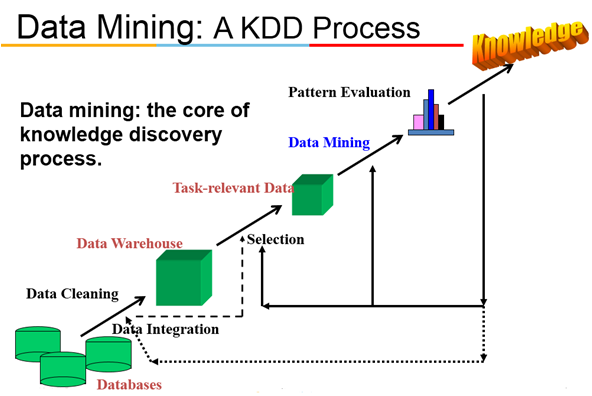
\includegraphics[scale=1.2]{kdd.png}
\caption{\label{fig:subBDDs1}Overview of steps in KDD process}
\end{figure}
\pagebreak
\section{Data Mining in Healthcare}
In today's world, healthcare information systems are capturing data in databases for research and analysis in order to assist in medical decisions. However, the data being stored is increasing on a daily basis and the data available today is in zillions and not in millions. Therefore, the process of extracting useful information is becoming difficult but data mining holds great potential for the healthcare industry to enable health systems to systematically use data and analytics to identify inefficiencies and best practices that improve care and reduce costs. Some experts believe the opportunities to improve care and reduce costs concurrently could apply to as much as 30\% of overall healthcare spending. By performing data analysis clinicians and medical researchers should be able to diagnose the disease and also assist medical science in the development of curative medicines.
\section{Introduction to Diabetes}
Recently it is observed that the number of people suffering from Diabetes Mellitus (DM), commonly referred to as diabetes, is increasing at an alarming rate and unfortunately, it is observed that a lot of young children suffer from diabetes. Diabetes is a group of metabolic disorders in which there are high blood sugar levels over a prolonged period. Symptoms of high blood sugar include frequent urination, increased thirst, and increased hunger. If left untreated, diabetes may lead to a lot of complications. Acute complications include diabetic ketoacidosis, hyperosmolar hyperglycemic state, or death. Serious long-term complications include cardiovascular disease, stroke, chronic kidney disease, foot ulcers, and damage to the eyes. Diabetes is due to either the pancreas not producing enough insulin or the cells of the body not responding properly to the insulin produced. There are three main types of diabetes mellitus:
\begin{itemize}
\item \textbf{Type 1} results from the pancreas's failure to produce enough insulin. This form was previously referred to as insulin-dependent diabetes mellitus (IDDM) or ``juvenile diabetes". The cause is unknown.
\item \textbf{Type 2} begins with insulin resistance, a condition in which cells fail to respond to insulin properly. As the disease progresses a lack of insulin may also develop. This form was previously referred to as non insulin-dependent diabetes mellitus (NIDDM) or adult-onset diabetes. The most common cause is excessive body weight and not enough exercise. 
\item \textbf{Gestational diabetes} is the third main form and occurs when pregnant women without a previous history of diabetes develop high blood sugar levels.
\end{itemize}
\par\noindent
Prevention and treatment involve maintaining a healthy diet, regular physical exercise, a normal body weight, and avoiding use of tobacco. Control of blood pressure and maintaining proper foot care are important for people with the disease. Type 1 must be managed with insulin injections. Type 2 may be treated with medications with or without insulin. Insulin and some oral medications can cause low blood sugar. Gestational diabetes usually resolves after the birth of the baby.\par\noindent
\section{Dataset}
The dataset used in this study is “The Pima Indians Diabetes Data Set” which was taken from the UCI Machine Learning Repository. The original owner of this data set is the National Institute of Diabetes and Digestive and Kidney Diseases. One major constraint placed on this dataset is that all patients selected are females at least 21 years old of Pima Indian heritage. In this project we will be building 4 classification models namely ANN, ID3, CART and C4.5.\par \noindent
The following are the parameters considered in this dataset and a brief detail pertaining to it.
\begin{itemize}
\item \textbf{Pregnancies:} Number of times pregnant
\item \textbf{Glucose:} Plasma glucose concentration- 2 hours in an oral glucose tolerance test
\item \textbf{BloodPressure:} Diastolic blood pressure (mm Hg). It indicates the pressure in the arteries when the heart rests between beats.
\item \textbf{SkinThickness:} Triceps skin fold thickness (mm). A value used to estimate body fat, measured on the right arm halfway between the olecranon process of the elbow and the acromial process of the scapula.
\item \textbf{Insulin:} 2-Hour serum insulin (mu U/ml)
\item \textbf{BMI:} Body mass index (weight in kg/(height in m)\^2)
\item \textbf{DiabetesPedigreeFunction (DPF):} DPF provides some data on diabetes mellitus history in relatives and the genetic relationship of those relatives to the patient. This measure of genetic influence gives an idea of the hereditary risk one might have with the onset of diabetes mellitus.
\item \textbf{Age:} Age (years)
\item \textbf{Outcome:} Class variable (0 or 1)
\end{itemize}
The summary statistics of the dataset attributes is tabulated in Table 1.1.
\pagebreak
\begin{table}[h]
\begin{center}
\begin{tabular}{| c | c | c | c | c | c |}
  \hline
  \textbf{Attribute} & \textbf{Type} & \textbf{Mean} & \textbf{Std} & \textbf{Min} & \textbf{Max} \\[2.5ex]
  \hline

  Pregnancy & Quantitative Discrete & 3.845 & 3.37 & 0 & 17  \\[2.5ex]
  \hline
  Glucose & Quantitative Continuous & 120.895 & 31.973 & 0 & 199  \\[2.5ex]
  \hline
  BP & Quantitative Continuous & 69.105 & 19.356 & 0 & 122  \\[2.5ex]
  \hline
  Skin Thickness & Quantitative Continuous & 20.536 & 15.952 & 0 & 99  \\[2.5ex]
  \hline
  Insulin & Quantitative Continuous & 79.799 & 115.244 & 0 & 846  \\[2.5ex]
  \hline
  BMI & Quantitative Continuous & 31.993 & 7.884 & 0 & 67.1  \\[2.5ex]
  \hline
  DPF & Quantitative Continuous & 0.472 & 0.331 & 0.078 & 2.42  \\[2.5ex]
  \hline
   Age & Quantitative Discrete & 33.241 & 11.76 & 21 & 81  \\[2.5ex]
  \hline 
\end{tabular}
\end{center}
\caption{\label{table:TT}Summary statistics of attributes in the dataset}
\end{table}
\section{Proposed System}
This project aims in building a model to classify if a person has  diabetes or not
using ANN and decision tree algorithms namely--ID3, C4.5, CART and compare the results obtained in both the models. Evaluation metrics like accuracy, error rate, sensitivity, specificity and precision will be calculated. The modules split-up of the proposed project is represented in Figure 1.2.
\begin{figure}[h]
%\vspace{-3.8in}
\centering %\offinterlineskip
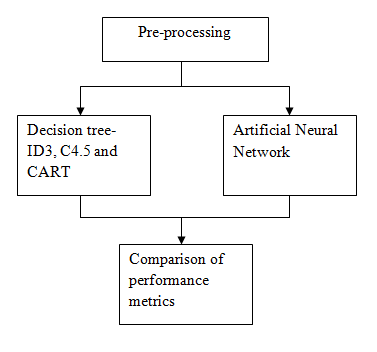
\includegraphics[scale=1.15]{modules.png}
\caption{\label{fig:subBDDs1}Modules split-up}
\end{figure}
\pagebreak
\section{Organization of the report}
In this report we start by introducing the premise of data mining, and diabetes. We then proceed to elucidate on our dataset and the proposed system. Chapter 2 covers the excerpts from our extensive literature review. The pre-processing techniques that were applied are discussed in Chapter 3 followed by the building of various classifiers. In our last chapter we summarize our results and discuss about the future scope of our above presented project.

 % INTRODUCTION

\chapter{LITERATURE SURVEY} 
Extensive research has been done in the area of classification and prediction of diabetes.
\section{Decision Tree}
Decision tree method was used to predict diabetes among patients with and without diabetes [2] using Pima Indian dataset taken from UCI Machine Learning Repository which has data collected from females over the age of 21. Two phases were involved. In the first phase data pre-processing techniques like attribute identification and selection, handling missing values and numerical discretization is applied. The transformed data is then used for classification based on the J48 algorithm which is a decision tree learner and an implementation of Quinlan C4.5 in Weka Knowledge Explorer, in phase two. The same software was used to test the model constructed by applying 10-fold cross validation and an overall accuracy of 78.1768\% was achieved from the results. Only one decision tree algorithm- J48 was used to classify the patients in the dataset. Moreover, only the accuracy and error rates were considered for evaluation of the performance.\par\noindent
RapidMiner tool was used in PIMA Indian dataset [6]. Missing value for the attributes Plasma-Glucose, DiastolicBP, and BMI were removed followed by outlier analysis. Numerical attributes were discretized before normalization. After normalizing the data, two predictive models are built namely decision tree and ID3.
A decision tree can be learnt by splitting the source data set into subsets based on an attribute value test. This process is repeated on each derived subset in a recursive manner. The recursion is completed when splitting is either non-feasible or a singular classification can applied to each element of the derived subset. A random forest classifier uses a number of decision trees, in order to improve the classification rate. It was found that this method gives an accuracy of 72\%.
The ID3 Algorithm adopts a greedy (i.e., non-backtracking) approach where decision trees are recursively constructed in a top-down divide and conquer manner. It starts with a training set of tuples and associated class labels. The training set is recursively partitioned into smaller subsets as the decision tree is being built and this method produces an accuracy of 80\% which is greater than the previous method by 8\%. \par\noindent  
Modified version of the ID3 algorithm [8] was used to classify the dataset which is continuous and bound into a specific range. By dividing a continuous feature into k intervals, the ID3 algorithm will create a decision tree that can work well on the floating point value data set, which cannot be classified in the original ID3. Pima dataset was split into a 75 is to 25 ratio and selects k values as 3, 6, 9, 12, 15, 18 and 20. It is observed that as the number of intervals increases, the decision tree has more choices for the samples to fall into their appropriate categories and hence decreases the error rate of the decision tree learning. However, at a specific number of k (k=12), the decision tree seems to get into the optimal state. The error rate of the decision tree, which has a value of k exceeding the best point, does not decrease as in the previous k. As a result, the error rates for k value 15, 18 and 20 are higher than that of 12.
As the modified ID3 continues increasing the value of k beyond the finest point, the error rate gradually increases. It indicates that there must be an appropriate value of k for a particular feature. The suitable value of k for the Pima Indian diabetes problem, should be around 12 and the accuracy was found to approximately 65\%.

\section{ANN}
Classification of diabetes data was performed on Pima Indian Diabetes dataset using Complex-Valued Neural Networks (CVNN) and Real-Valued Neural Networks (RVNN) based parametric modelling approaches [1]. Complex data normalization technique converts the real valued input data (RVD) to complex valued data (CVD). CVNNs learn the relationship between the input and output data during training and the Complex-valued Autoregressive (CAR) model is extracted from the complex-valued weights and coefficients of trained network. Finally, classification of the CAR or RVAR model coefficients is performed. Further, the effect of data normalization techniques, activation functions, learning rate, number of neurons in hidden layer and the number of epoch is studied and evaluated in this paper.

The first stage is data formatting (structural representation of the data in accordance to the model format) and normalization (band limiting of the data). Complex data normalization converts RVD to CVD and both kinds of data are studied. The data normalization techniques used are- z-score normalization (NT1), min-max data normalization (NT2), complex data normalization (NT3) and unitary data normalization (NT4). NT3 data normalization maps input RVD to a complex valued interval [0,$\pi$] and retains the relational and spatial properties that exist between two entities in RVD.
The ANN-based AR model classification technique is developed.
The model coefficients obtained from the trained network is grouped into regions, and hence the model output classifier is built.
The performance analysis in this paper include- True Positive (TP), True Negative (TN), False Positive (FP), False Negative (FN), Accuracy (Acc) and Time of Completion (TOC).
Effect of data normalization, number of neurons in the hidden layer, learning rate, number of epoch and activation function on the accuracy of the proposed model is observed.
It was found that the accuracy obtained using hyperbolic tangent is better than that obtained using sigmoid activation function.
The proposed model performed better using complex data normalization technique with hyperbolic tangent (tanh) as activation function.
The use of very low learning rate increased the TOC while high learning rate led to instability in the algorithm.
Increasing the number of neurons in the hidden layer did not have a significant effect on accuracy of the model for tanh activation function using NT1, NT2 and NT3 techniques. For NT4, increasing the number of neurons in the hidden layer increased the accuracy.
It was observed that, increasing the number of epochs led to an increase in TOC without affecting accuracy.
TOC using tanh activation function was always greater than TOC using sigmoid for all data normalization techniques, implying a trade off between accuracy and TOC in using tanh or sigmoid.
It was concluded that the proposed ANN-based AR model produced accuracy in the range of 80.65\%-81\% which compare favorably with existing classification techniques for the same dataset. \par \noindent
Four models namely Artificial Neural Network (ANN), Decision tree (DT), Support Vector Machine (SVM) and Logistic Regression (LR) was performed on Pima Indian diabetes dataset [3]. The first stage of pre-processing used was to discard the cases having one or more missing attribute values from the original 768 cases. Then the remaining missing values are imputed using K-Nearest Neighbor (KNN) algorithm. After imputing the data outliers are detected using box plot and the outliers are eliminated. Following which the hidden patterns in the dataset are extracted using K-means algorithm and the misclassified samples are eliminated and the correctly classified samples are given as inputs to the ANN, DT, SVM, LR with a 70-30 split. The developed models cascaded k-means combined with LR and k-means combined with ANN give an accuracy above 98\%. The model k-means and SVM achieved an accuracy 97.13\% and the model K-means and DT achieved an accuracy of 97.99\%. As compared with accuracy the proposed model cascaded k-means and LR is best among the methods considered. \par \noindent   
A hybrid Adaptive Neuro-Fuzzy Inference System (ANFIS) was used for classifying diabetes in the Pima Indians Diabetes dataset [5]. It was implemented using ANFIS Fuzzy Logic Toolbox and MATLAB Toolbox. The performance measures were analyzed in terms of specificity, precision and sensitivity.
ANFIS is a hybrid adaptive neural network that has the capability to adjust the membership functions and the consequent parameters during learning process, by applying an optimization method. In this case, mean square error between current neuro-fuzzy system and its proposed output was used as the minimized criteria function.
A five-layer ANFIS structure had the following functions:\newline
Layer 1: Every node was an adaptive node with a node function \newline
Layer 2: Every node was fixed, whose output was a product of all incoming signals and represented the firing strength of a rule. \newline
Layer 3: Every node was a fixed node. The ith node calculated the ratio of the ith rule’s firing strength to the sum of all rule’s firing strengths. \newline
Layer 4: Every node was an adaptive node with a node function. \newline
Layer 5: Had a single, fixed node which computed the overall output as summation of all incoming signals. \newline
The training set used had 80\% of the data, and the test set had 20\% of data. Linear function coefficients were calculated by least squares method RMS. Error signals were back-propagated and the antecedent parameters of membership function were updated using gradient descent method.
The training process yielded the rule base. The dataset selected for testing included six variables- Plasma Glucose Concentration, Diastolic Blood Pressure, Triceps skin fold thickness, 2-Hour serum insulin, Body mass index and Diabetes pedigree function.
The quality of classifier was measured from confusion matrix that contains, True positive (TP), True negative (TN), False positive (FP) and False negative (FN) cases. Based on these values accuracy, sensitivity, specificity and precision values were computed. It was observed that the proposed neural network produced an accuracy of 85.35\% for training data and 84.27\% for testing data. \par \noindent
Various pre-processing techniques were used to compare the performance of Artificial Neural Network (ANN) to classify the patients in Pima Indian dataset [7]. The impact of pre-processing is highly relevant in this context because medical datasets generally have missing values but ANNs require complete set of data for accurate classification. Computer simulations were carried out using MATLAB to analyze the performance of four approaches of pre-processing namely- (1) omit samples, (2) replace with zeros, (3) replace with mean and (4) replace with KNN with respect to epochs. Accuracy was tremendously improved when using KNN and mean with PCA preprocessing method. \par \noindent
Two models, namely, multilayer neural network trained by Levenberg-Marquardt (LM) algorithm and a probabilistic neural network were built on Pima Indian diabetes dataset [10].
The first stage was construction of a multilayer neural network (MLNN) structure trained by LM algorithm. The widely recognized back-propagation (BP) algorithm suffers from a slow convergence rate, and leads to suboptimal solutions because it applies the steepest descent method to update the weights. Hence, LM algorithm which provides faster convergence and better estimation results was used. However, LM can cause memorization effect when the overtraining occurs. This effect decreases the generalization and performance may not be improved for untrained test sets. In order to address this drawback, the study proposed to determine the optimum trained neural network using the maximum accuracy value of the test data.
At the second stage, a probabilistic neural network (PNN) was built. It is a model based on competitive learning with ‘winner takes all’ strategy and the core concept based on multivariate probability. The PNN used feature vector as eight-dimensional real valued input vector, with a single hidden layer (radial basis layer) which are fully interconnected to an output layer of two units which are indices of two classes.
Two kinds of validation techniques were used. The conventional one training set and one test set validation; and 10-fold cross-validation technique was applied and accuracy was compared to other neural network models. For the conventional validation method, the first 576 cases were used as the training set and the remaining 192 cases were used as the test set. In k-fold cross-validation method, the dataset is divided into k mutually exclusive subsets. The training and testing is done k times. In each iteration one of the folds is taken as test data and remaining (k-1) folds are used as training set. Thus, k different test results are obtained for each train-test configuration and average of these results give the test accuracy of the algorithm.
An accuracy of 79.62\% was obtained for MLNN with LM and 78.05\% was obtained with PNN when 10-fold cross-validation was used. The same algorithms (i.e. MLNN with LM and PNN) gave 82.37\% and 78.13\% accuracies respectively with conventional validation technique.

\section{General}
The performance of multiple ensemble techniques like Majority voting, Adaboost, Bayesian Boosting, Stacking and Bagging were compared [4]. Three types of decision trees- ID3, C4.5 and CART were used as base classifiers. Two benchmark datasets from UCI and Biostat repository were used and the experimental results show that Bagging ensemble technique shows better performance when compared to a single classifier as well as other ensemble techniques. Since ensemble classifiers are more accurate in performance and prediction than standalone classifiers and that they produce more flexible structure, it can be applied in the field of data mining for diabetes diagnosis. The methodology proposed involves implementation of the three decision trees- (ID3, C4.5 , CART) and use these as a base classifier for various ensemble classifiers which generate different performance while evaluating parameters like accuracy, sensitivity, specificity and f-measure using RapidMiner tool. A future scope of applying the aforementioned technique for other disease datasets like breast cancer, heart disease and liver disease was provided. Moreover, heterogeneous base classifiers can be applied to increase the performance. \par \noindent
A survey of various data mining methods applied to diabetes data analysis and prediction of the disease was discussed [9]. It describes three broad methodologies to approach the same. Firstly, several association rule based algorithms in this context are as follows:
\begin{itemize}
\item A new approach to generate association rule on numerical data by applying pre-processing techniques like equal interval binning and then applying Apriori Association Rule algorithm to generate the rules.
\item An advanced and reliable technique to identify risk factors behind the diabetes to generate association rules and identify the relationship between diabetes and other diseases.
\item Combination of decision tree and association rule approach to build different decision trees, convert them into different set of rules and then further reduce and filter it. The final conclusion is that the set of rules from decision tree was much smaller than the results of association rules.
\item Theory of association rule of Diabetes Mellitus (DM) patients data with renal, Ophthalmic, Neurological and Peripheral Circulatory complications.
Secondly, various clustering and classification based algorithms for diagnosis of diabetes are as follows:
\item Combination of K-means clustering with various classification algorithms like SMO (Simple Minimal Optimization), Naive Bayes, Bagging, AdaBoost, J48, Rotation Forest and Random Forest.
\item Hybrid model for classifying PIMA Indian dataset. Identify datasets and incorrectly classified instances are eliminated using K-means clustering. C4.5 decision tree is done on correctly clustered instances and resultant dataset is tested using 2 methods- dividing training and testing data into 60-40 ratio and 10-fold cross validation. This method improves accuracy by an order of 19.50\% of classification compared to decision tree C4.5 alone with unprocessed data.
\item Research done on 3 technique- Expectation Maximization (EM), H-means clustering and Genetic Algorithm(GA) on PIMA dataset.
\end{itemize}
Thirdly, other methods like RapidMiner tool, CART, Neural Network and Artificial MetaPlasticity on Multilayer Perceptron (AMMLP) for the purpose of diabetes prediction and diagnosis were discussed. Finally it can be concluded that from analysis of various presentations and studies done by other researches it is evident that occurrence of diabetes is having a strong relation with
\begin{enumerate}
\item Diseases like wheeze, edema etc.
\item Female pregnant
\item Increase of age
\end{enumerate}
Data mining techniques have to be done more intrinsically to relate diabetes to other diseases for accurate and early detection as a part of future scope. \par \noinent
A homogeneous ensemble technique was used [11]. It ascertains that the ensemble models accuracy is way better than any algorithm alone. The ensemble method used is random forest. The algorithm, performs better when the number of attributes or features is greater than the number of tuples themselves. Random forest algorithm constructs several randomized decision trees and aggregates their predictions for improved accuracy. A fair idea about the unrelated features like Total Cholesterol, High Density Lipoprotein, Stabilized Glucose, High Density Lipoprotein, the Cholesterol/HDL Ratio and the First Systolic Blood Pressure was given, which paves way for dimensionality reduction. Data like age, weight, height, hip, and waist have been discretized. Gini index has been used to determine the split point. The final result is presented based on majority voting. Based on individual decision trees, rules and useful relationships may be extracted. Another interesting observation made is the accuracy with respect to data scale. It is seen that random forest method is consistently improving with increase in the proportion of input data. Thus, random forest is suitable for sufficiently large data sets. A homogeneous ensemble technique was discussed, however it is possible to obtain better results using heterogeneous alternatives.

 % LITERATURE SURVEY

\chapter{PRE-PROCESSING} 
Various preprocessing techniques were applied to the given data set, and all the proposed models were built on this data. The PIMA Indian Diabetes dataset was found to have 0 values for certain attributes, which doesn't comply with common sense in real life. Thus, these ``0 values" were treated as missing data, and were handled using different methodologies. Specifically, with respect to our dataset, the following were the attributes with the above mentioned characteristics:
\begin{itemize}
    \item Glucose
    \item Blood Pressure
    \item Skin Thickness
    \item Insulin
    \item BMI
\end{itemize}

The pre-processing techniques employed on the data can be broadly classified into two categories:
\begin{itemize}
    \item Handling the missing values ( “0 values” in the above specified attribute list)
    \item Normalizing the data

\end{itemize}

\section{Methodologies Employed}
Techniques for handling missing data  include:
\begin{itemize}
    \item \textbf{Filling the zero values with mean:}
The attributes with missing values were first replaced with ``nan" ( not a number ), and ``nan" was subsequently replaced with the mean of each corresponding attribute.
    \item\textbf{Filling the zero values with median:}
The attributes with missing values were first replaced with ``nan" ( not a number ), and ``nan" was subsequently replaced with the median of each corresponding attribute.

\item \textbf{Dropping the rows containing attributes with these missing values:}
The attributes with missing values were first replaced with ``nan" ( not a number ), and rows with ``nan" were subsequently dropped. The size of the dataset reduced to almost 50\% of the initial size.

\item \textbf{Using the k-nearest neighbour classifier to fill appropriate values:}
A KNN model was built for each and every attribute with missing values separately. These models were used to predict the probable values for the corresponding attribute's missing data.
\end{itemize}

Normalization of data was done using PCA (Principal Component Analysis), and the number of resultant components was fixed as 8, which is the same as the number of input attributes. The various preprocessing techniques against the different models along with evaluation parameters have been tabulated in Table 3.1.


\begin{adjustbox}{angle=90}
\scalebox{0.87}{
    \begin{tabular}{|c|c|c|c|c|c|c|}
    \hline
    \textbf{MODEL} & \textbf{PRE PROCESSING} & \textbf{ACCURACY} & \textbf{SENSITIVITY} & \textbf{SPECIFICITY} & \textbf{PRECISION} &	\textbf{ERROR RATE} \\ 
    \hline     
    \multirow{ID3} & Mean & 79.87 & 70.21 & 84.11 & 66 & 20.13\\
    & Median & 74.68 & 72.34 & 75.7 & 56.67 & 25.32\\
    & Dropping & 75.95 & 52 & 87.03 & 65 & 24.05\\
    & KNN & 80.51 &	61.7 & 88.78 & 70.73 & 19.49\\
    & KNN + PCA & 68.18 & 59.57 & 70.96 & 48.27 & 31.82\\
    \hline
    \multirow{CART} & Mean & 78.57 & 65.95 & 84.11 & 64.58 & 21.43\\
    & Median & 78.57 &	65.95 &	84.11 &	64.58 &	21.43\\
    & Dropping	& 78.48 & 60 & 87.03 &	68.18 &	21.52\\
    & KNN &	72.07 &	57.44 & 78.5 &	54 &	27.93\\
    & KNN + PCA	& 68.83 & 61.7 & 71.96 & 49.15 & 31.17\\
    \hline
    \multirow{C4.5} & Mean & 77.27 & 62.96 & 85 & 69.39 & 22.73\\
    & Median & 77.27 & 62.96 & 85 &	69.39 &	22.73\\
    & Dropping & 66.67 & 46.15 & 76.92 & 50 & 33.33\\
    & KNN &	77.27 &	62.96 &	85 & 69.39 & 22.73\\
    \hline
    \multirow{ANN} & Mean & 81.17 &	76.59 &	83.17 &	66.66 &	18.83\\
    & Median &	80.52 &	59.57 &	89.72 & 71.79 &	19.48\\
    & Dropping & 81.01 & 68	& 87.04 & 70.83 & 18.99\\
    & KNN &	74.03 &	65.96 &	77.57 & 56.36 &	25.97\\
    & KNN + PCA	& 81.82 & 48.94 & 96.26 & 85.18 & 18.18\\
    \hline
    \end{tabular}}
    
\end{adjustbox}
\captionof{table}{All preprocessing techniques, models and evaluation metrics}
%\newpage
\clearpage
\begin{figure}[h]
%\vspace{-3.8in}
\centering %\offinterlineskip
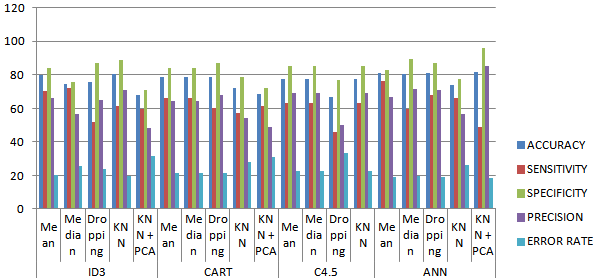
\includegraphics[scale=1.15]{sumprp4.PNG}
\caption{\label{fig:subBDDs1}Summary of all pre-processing techniques, models and parameters}
\end{figure}
\par \noindent The Table 3.1 has been briefly summarized in Figure 3.1.
%\pagebreak
Figure 3.2 summarizes the results obtained from the top two pre-processing techniques for each model.
\begin{figure}[h]
%\vspace{-3.8in}
\centering %\offinterlineskip
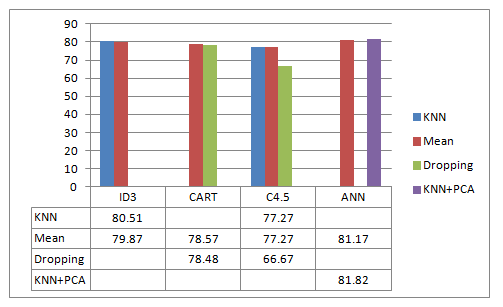
\includegraphics[scale=1.15]{topprp.PNG}
\caption{\label{fig:subBDDs1}Top two pre-processing technique for all models
based on accuracy
}
\end{figure}
\pagebreak
\section{Consensus}
In the above tabulation, the best pre-processing technique (decided based on the model accuracy) for a model, it can be observed that \textbf{mean} is the only preprocessing technique that occurs as either the best or the second-to-best preprocessing method for all the models. Hence filling the missing values with mean was the only data preprocessing technique, that was applied to our dataset. % DESIGN
\chapter{BUILDING THE VARIOUS CLASSIFIERS}
The major idea behind this project is to build different classification models for the PIMA Indian Diabetes dataset, and to compare these models based on various evaluation parameters like accuracy, sensitivity, specificity, precision and error rate. In this regard, we intend to classify the data using decision tree algorithms like ID3, CART, C4.5 and ANN.
In the upcoming subchapters, the algorithmic aspect of these classifiers will be detailed.

\section{Decision Trees}
A decision tree is a decision support tool that uses a tree-like graph or model of decisions and their possible consequences, including chance event outcomes, resource costs, and utility. It is a flowchart-like structure in which each internal node represents a test on an attribute, each branch represents the outcome of the test, and each leaf node represents a class label (decision taken after computing all attributes). The paths from root to leaf represent classification rules.

A decision tree consists of three types of nodes:
\begin{enumerate}
    \item \textbf{Decision nodes} – typically represented by squares
    \item \textbf{Chance nodes} – typically represented by circles
    \item \textbf{End nodes} – typically represented by triangles
\end{enumerate}

The pseudo code of decision tree is followed as:-

\begin{figure}[h]
%\vspace{-3.8in}
\centering %\offinterlineskip
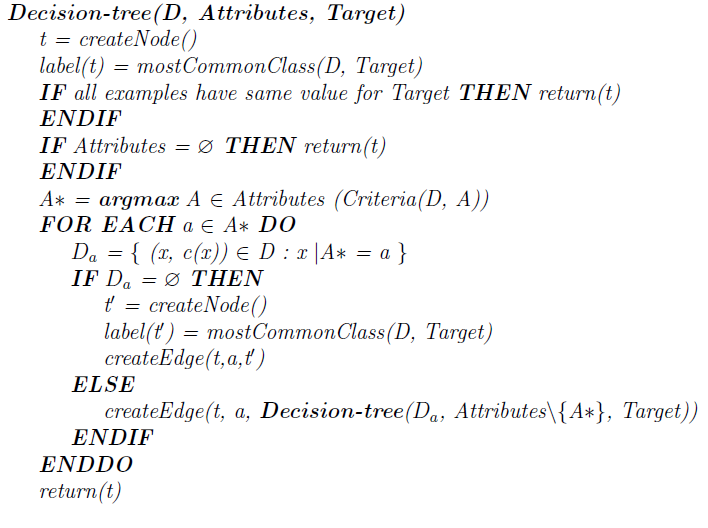
\includegraphics[scale=0.97]{dtcode.png}
\end{figure}
\pagebreak

The function \textbf{Criteria()} is the one that distinguishes the decision tree algorithms from each other. For all the models of decision tree, a 80-20 split was done on the dataset for training and testing the built model.

\subsection{ID3}
\begin{itemize}
    \item Select the attribute with the highest information gain.
    \item Let $p_i$ be the probability that an arbitrary tuple in $D$ belongs to class $C_i$ estimated by $ |C_{i,D}| / |D| $
    
    \newpage
    
    
    \item Expected Information (entropy) needed to classify a tuple in $D$
  
    \[ Info(D) = -\sum_{i=1}^{m} p_i \hspace{0.3cm} log_2(p_i) \]
    
    \item Information needed, after using $A$ to split $D$ into $v$ partitions to classify $D$
    
    \[ Info_A(D) = \sum_{j=1}^{v} \hspace{0.15cm} (|D_j| / |D|)
    \hspace{0.12cm} X \hspace{0.12cm} Info(D_j) \]
    
    \item Information gained by branching on attribute $A$
    
    \[ Gain(A) = Info(D) \hspace{0.12cm} - \hspace{0.12cm} Info_A(D)      \]
    
\end{itemize}

Computing Information gain for continuous-value Attributes:
\begin{itemize}
    \item Let attribute $A$ be a continuous value attribute
    \item The best split point for $A$ must be determined:
    \begin{itemize}
        \item Sort the value of $A$ in increasing order
        \item Typically, the midpoint between each pair of adjacent values is   considered as a possible split point
        \item $ (a_i + a_{i+1}) / 2 $ is the midpoint between the values of $ a_i $ and $ a_{i+1} $
        \item The point with the minimum expected information requirement for $A$ is selected as the split-point for $A$
    \end{itemize}
\end{itemize}
\newpage
Figure 4.1 visualizes the pruned version of our ID3 decision tree after training the model. It was constructed using mean for handling missing values. 
\vspace{0.27in}
\begin{figure}[h]
\centering 
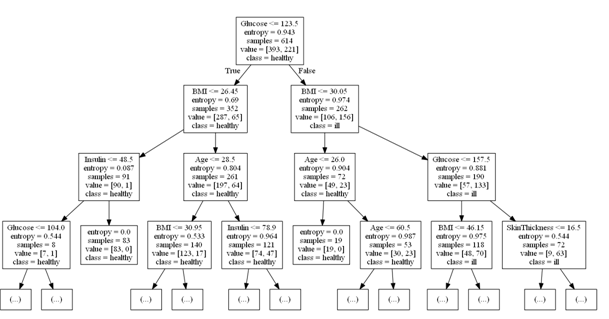
\includegraphics[width=7in,height=5in]{id3.PNG}
\caption{\label{fig:subBDDs1}ID3 decision tree}
\end{figure}
\newline
20\% of the dataset, i.e. 154 samples were used to validate the constructed decision tree. Figure 4.2 and 4.3 represents the output we obtained after building and testing our model.
\clearpage
\begin{figure}[h]
\centering
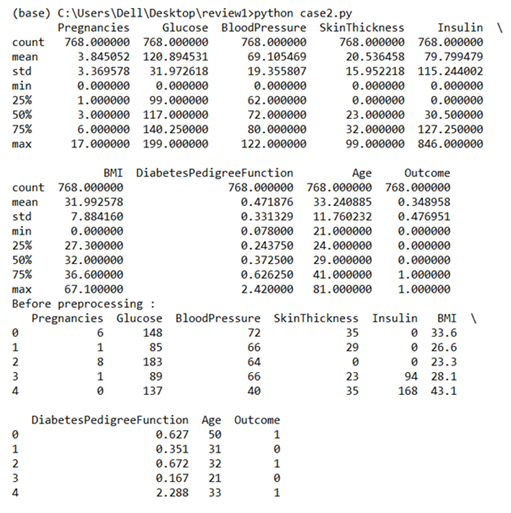
\includegraphics[scale=1.2]{sumbfprp.PNG}
\caption{\label{fig:subBDDs1}Summary of dataset before preprocessing}
\end{figure}
\pagebreak
\clearpage
\pagebreak
\begin{figure}[h]
\centering 
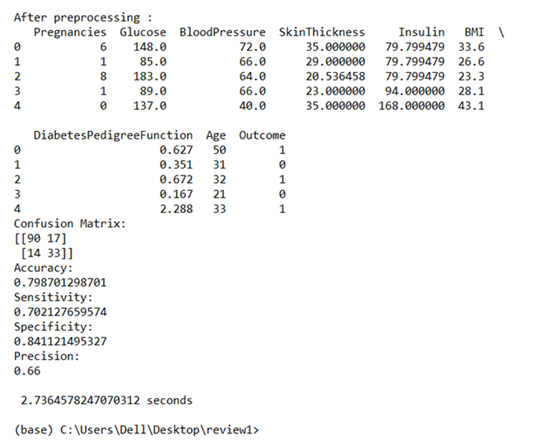
\includegraphics[scale=1.2]{dsfprp.PNG}
\caption{\label{fig:subBDDs1}Dataset after pre-processing and evaluation metrics}
\end{figure}
\pagebreak
\clearpage
\subsection{C4.5}
C4.5 (a successor of ID3) uses gain ratio to overcome the problem (normalization to information gain)
\[SplitInfo_A(D) = -\sum_{j=1}^{v} \frac{|D_j|}{|D|}\hspace{0.12cm} X \hspace{0.12cm}log_2(\frac{|D_j|}{|D|}) \]
\[GainRatio(A) = Gain(A)/SplitInfo(A)\]
\par \noindent
The attribute with the largest GainRatio is selected as the Splitting  Attribute.
For, J48 (Quinlan C4.5) to be implemented, attributes need to be categorized prior to training the model. So, we referred the method proposed in study [2] to categorize the dataset variables. The Table 4.1 summarizes the splitting criteria used for discretizing each attribute.
\begin{table}[h]
\begin{center}
\begin{tabular}{| c | c |}
  \hline
  \textbf{Attribute} & \textbf{Split Criteria} \\[0.85ex]
  \hline
  Pregnant & low(0,1), medium(2,3,4,5), high($>$6) \\[0.85ex]
  \hline
  Glucose & low($<$95), medium(95-140), high($>$140) \\[0.85ex]
  \hline
  Blood Pressure & normal($<$80), normal-high(80-90), high($>$90) \\[0.85ex]
  \hline
  BMI & low($<$24.9), normal(25-29.9), obese(30-34.9), severely-obese($>$35) \\[0.85ex]
  \hline
  DPF & low($<$0.5275), high($>$0.5275) \\[0.85ex]
  \hline
  Age & range-1($<$28.5), range-2($>$28.5) \\[0.85ex]
  \hline
\end{tabular}
\end{center}
\caption{\label{table:TT}Criteria for categorizing attributes in dataset}
\end{table}
\par \noindent
Since study [2] deleted 2 attributes namely, Skin Thickness and Insulin, the discretization for these two variables, was done using qcut function.  It is a Quantile-based discretization function provided by the Pandas library in Python.\par \noindent
Figure 4.4 visualizes the C4.5 decision tree constructed after categorizing the attributes in the Pima dataset using mean for handling missing values.
\begin{figure}[h]
\centering
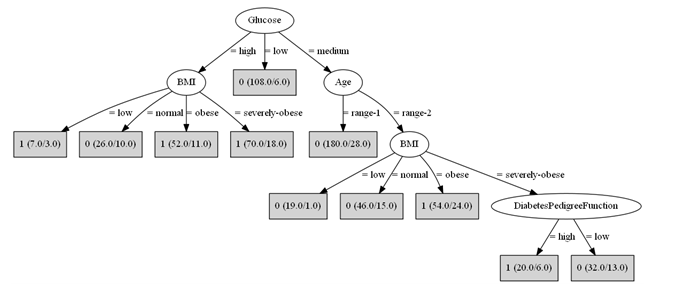
\includegraphics[scale=1.0]{c45.PNG}
\caption{\label{fig:subBDDs1}C4.5 Decision tree}
\end{figure}
\par \noindent
\newline 
20\% of the dataset, i.e. 154 samples were used to validate the constructed decision tree. Figure 4.5 represents the output we obtained after building and testing our model.
\begin{figure}[h]
\centering
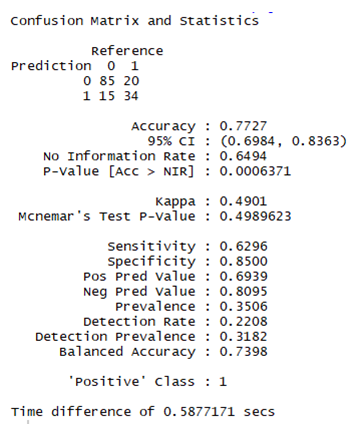
\includegraphics[scale=1.0]{c45eval.PNG}
\caption{\label{fig:subBDDs1}C4.5 evaluation metrics}
\end{figure}
\pagebreak



\subsection{CART}
\begin{itemize}
    \item If a data set D contains examples from n classes, gini index is defined as:
    \[ gini(D) = 1 - \sum_{j=1}^{n} p_j^2    \]
    \item If a data set D is split on A into two subsets D1 and D2, the gini index is defined as:
    \[ gini_A(D) = (|D_1| / |D|)gini(D_1) \hspace{0.12cm} + \hspace{0.12cm} (|D_2| / |D|)gini(D_2)    \]
    \item Reduction in Impurity:
    \[ \Delta gini(A) = gini(D) \hspace{0.12cm} - \hspace{0.12cm} gini_A(D) \]
    \item The attribute that provides the smallest $ginisplit(D)$ (or the largest reduction in impurity) is chosen to split the node.
    \item This is enumerated for all the possible splitting points for each attribute.
\end{itemize}
The Figure 4.6 visualizes the pruned version of our CART decision tree.
\begin{figure}[h]
\centering
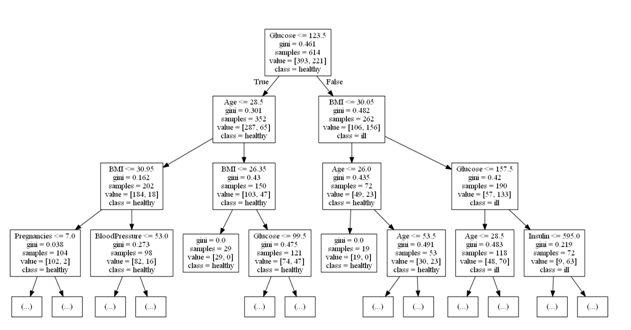
\includegraphics[width=7in,height=5in]{cart.PNG}
\caption{\label{fig:subBDDs1}CART Decision tree}
\end{figure}
\newpage
20\% of the dataset, i.e. 154 samples were used to validate the constructed decision tree. Figure 4.7 represents the output we obtained after building and testing our model.
\begin{figure}[h]
\centering
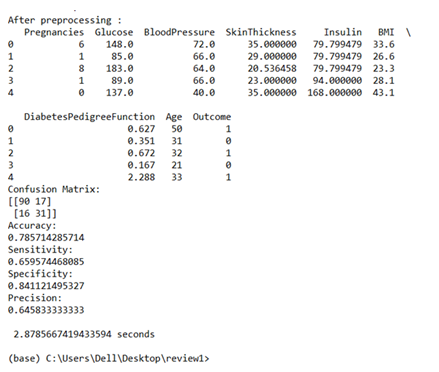
\includegraphics[scale=1.4]{carteval.PNG}
\caption{\label{fig:subBDDs1}CART evaluation metrics}
\end{figure}

\newpage
\section{ANN Algorithm}
Artificial Neural Networks are a computational tool modelled on the interconnection of the neuron in the nervous systems of the human brain and that of other organisms. They are composed of multiple nodes, which imitate biological neurons of human brain. The neurons are connected by links and they interact with each other. The nodes can take input data and perform simple operations on the data. The result of these operations is passed to other neurons. The output at each node is called its activation or node value. Each link is associated with weight. ANNs are capable of learning, which takes place by altering weight values.
\begin{figure}[h]
\centering
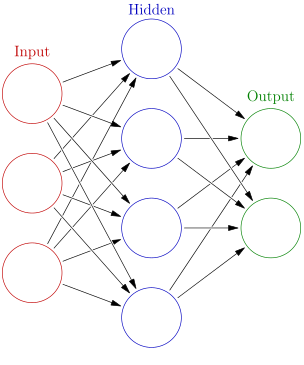
\includegraphics[scale=1.0]{ann.png}
\caption{\label{fig:subBDDs1}Struture of ANN}
\end{figure}
\par \noindent
There are two Artificial Neural Network topologies –
\begin{itemize}
\item \textbf{FeedForward ANN} - The information flow is unidirectional. A unit sends information to other unit from which it does not receive any information. There are no feedback loops.
\item \textbf{FeedBack ANN} - where, feedback loops are allowed.
\end{itemize}
\par \noindent
The ANN model that we have built for our data set has the following characteristics.
\begin{itemize}
\item We have built a feed-forward ANN with backpropagation.
\item One input layer, one hidden layer, and one output layer, each consisting of 12, 8, and 1 node(s) respectively. For convenience, from now on, we will refer to the input, hidden and output layers as i, h, and the o layers respectively.
\item The i, h, and the o layers use relu, relu, and sigmoid as their activation functions respectively.
\item Adam was used as the model optimizer.
\item Adam was used as the model optimizer.
\item The number of epochs ( the number of times for which the model sees the entire of the training data set ) was fixed to 1000.
\item The number of tuples per training batch ( batch size ) was fixed to 16.
\par \noindent
The impact of batch size was extensively studied by subjecting our Neural Network to various batch size values. The batch sizes considered are powers of 2 because of the efficient allocation of batches of dataset to the processors(or cores) in the system. The line chart built in Figure 4.9 summarizes the same.
\begin{figure}[h]
\centering
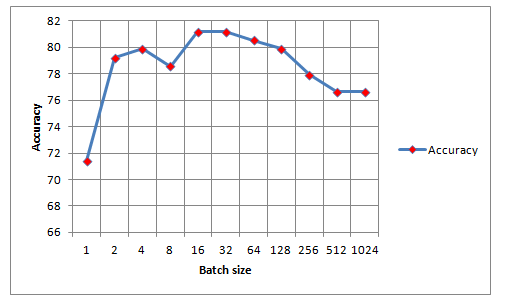
\includegraphics[scale=1.0]{batch.PNG}
\caption{\label{fig:subBDDs1}Impact of batch size}
\end{figure}
\pagebreak
From Figure 4.9, it’s clear that accuracy of ANN reaches its peak batch size of 16 and 32. Any value of batch size lower or higher gradually decreases the accuracy. Hence, our choice of 16 as batch size is well warranted for the constructed ANN.
\item 80\% of the entire dataset was used to train the model, and the rest was used to test the model.
\end{itemize}
\par \noindent
\newline
20\% of the dataset, i.e. 154 samples were used to validate the constructed decision tree. Figure 4.10 represents the output we obtained after building and testing our model.
\begin{figure}[h]
\centering
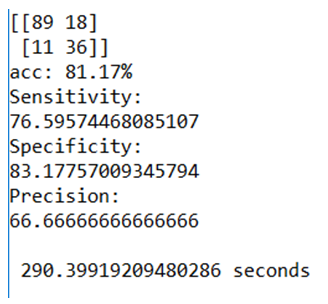
\includegraphics[scale=1.0]{anneval.PNG}
\caption{\label{fig:subBDDs1}ANN evaluation metrics}
\end{figure}
\pagebreak
\newline

\section{Evaluation Metrics}
Before training the models, the data set was randomly split into training and testing set. 80\% of the input data was used for training and the remaining 20\% was used for testing. The models are built by learning from training set and the unknown test set is used for computing evaluation metrics to analyze the quality of the models built.

\begin{itemize}
    \item The \textbf{confusion matrix} captures the information regarding the actual and predicted target class labels from the test set. The general structure of a confusion matrix is represented in Figure 4.11
    \newpage
    \begin{figure}[h]
    \centering
    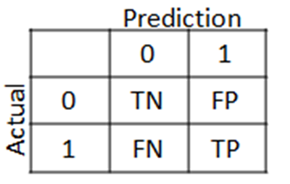
\includegraphics[scale=1.0]{cm.PNG}
    \caption{\label{fig:subBDDs1}Confusion Matrix}
    \end{figure}
    where,
    \begin{itemize}
        \item \textbf{TP} refers to the number of True Positive samples. They are test samples that are actually positive and classified as positive.
        \item \textbf{TN} refers to the number of True Negative samples. They are test samples that are actually negative and classified as negative
        \item \textbf{FP} refers to the number of False Positive samples. They are test samples that are actually negative but classified as positive
        \item \textbf{FN} refers to the number of False Negative samples. They are test samples that are actually positive but classified as negative
    \end{itemize}
\end{itemize}
Using the values from confusion matrix, the following evaluation metrics can be computed.
\begin{itemize}
    \item \textbf{Accuracy}: It is the ratio of number of samples correctly classified by the model and the total number of samples in the test set.
    \[
        Accuracy = \dfrac{TP+TN}{TP+TN+FP+FN}
    \]
    
    \item \textbf{Sensitivity}: It is the ratio of number of True Positive (TP) samples and the total number of positive samples in the test set.
    \[
        Sensitivity = \dfrac{TP}{TP+FN}
    \]
    
    \item \textbf{Specificity}:  It is the ratio of number of True Negative (TN) samples and the total number of negative samples in the test set.
    \[
        Specificity = \dfrac{TN}{TN+FP}
    \]
    \item \textbf{Precision}:  It is the ratio of number of True Positive (TP) samples and the total number of samples predicted as positive by the model.
    \[
        Precision = \dfrac{TP}{TP+FP}
    \]
\end{itemize} % IMPLEMENTATION
\chapter{CONCLUSION}
\section{Summary of the Results}

Section 2.2 has clearly justified the choice of mean as a viable pre-processing technique for handling missing values in the Pima Indian diabetes dataset. Hence, the comparison between the constructed classification models was done after handling the missing values with mean. The results obtained is tabulated in Table 5.1.

\newline
\begin{center}
\begin{tabular}{|c|c|c|c|c|}
\hline
\textbf{Parameter} &	\textbf{ID3} & \textbf{CART} & \textbf{C4.5} &	\textbf{ANN} \\
\hline
Accuracy & 79.87 & 78.57 & 77.27 & 81.17\\
\hline
Sensitivity &	70.21 &	65.95 &	62.96 &	76.59\\
\hline
Specificity &	84.11 &	84.11 &	85 & 83.17\\
\hline
Precision	& 66 &	64.58 &	69.39 &	66.66\\
\hline
\end{tabular}
\end{center}
\captionof{table}{Evaluation metrics for all models after pre-processing with mean}

\begin{figure}[h]
\centering
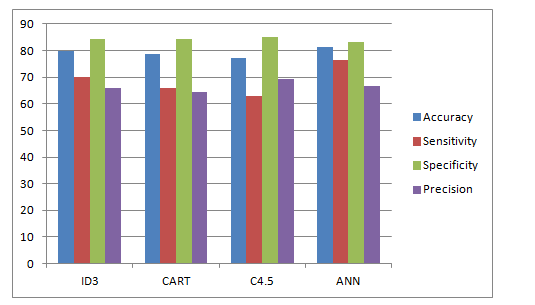
\includegraphics[scale=1.0]{evalmetall.PNG}
\caption{\label{fig:subBDDs1}Evaluation metrics for every model after
preprocessing with mean}
\end{figure}
\pagebreak

The bar chart visualization of the obtained results in Figure 5.1, shows that the ANN model has given the highest accuracy ahead of ID3, which emerged as the best decision tree model considering three evaluation metrics. It has also shown a significant increase of 6.38\% in the Sensitivity value when compared to ID3, which again had the best Sensitivity among the constructed decision trees. The Specificity value for ANN has slightly decreased (by 0.94\%) when compared to ID3. With respect to precision, it was C4.5 which gave the highest value of 69.39\%, ahead of ANN’s 66.66\%. Though, ANN has given slightly lower Specificity and Precision scores in comparison, it has clearly outperformed the other classification models, considering the other two metrics. Hence it can be rightly concluded that ANN has emerged as the best model when compared to the three decision tree variants, from an overall perspective.

\section{Future Work}
\begin{enumerate}
    \item The proposed project can be extended into an interactive application, say a Mobile or Web Application. The system can take values for various parameters as input and feed the constructed ANN. The output from Neural Network will correspond to either non-diabetic or diabetic (ie Outcome = 0 or 1). Hence, the predicted value will help the user know if he/she is classified as diabetic or not based on the parameters. 
    \item The subjects used for the Pima Indian Diabetes dataset are all women who are at least 21 years of age. Hence this data can be augmented with samples belonging to the male gender and people who are lesser than 21, which renders more generalization for the data as well as results. Moreover, all the diabetic patients in this dataset are affected by Type-2 diabetes. Hence, the same models can be constructed for a dataset pertaining to patients affected by Type-1 diabetes.
\end{enumerate} % CONCLUSION AND FUTURE WORK

\end{spacing}
\newpage
\appendix

%\addtotoc{REFERENCES}
%\input{References} 
%\bibliographystyle{plain}
%\bibliography{ref}
\begin{thebibliography}{99}
  \bibliographystyle{plain}
  
\bibitem[1]{1} Aibinu, A.M., Salami, M.J.E. and Shafie, A.A. (2010) `Application of modeling techniques to diabetes diagnosis', IEEE EMBS Conference on Biomedical Engineering and Sciences (IECBES), Kuala Lumpur, pp. 194-198.

\bibitem[2]{2} Al Jarullah, A.A. (2011) `Decision tree discovery for the diagnosis of type II diabetes', International Conference on Innovations in Information Technology, Abu Dhabi, pp. 303-307.

\bibitem[3]{3} Barale, M.S., Shirke, D.T. (2016) `Cascaded Modeling for PIMA Indian Diabetes Data' , International Journal of Computer Applications, 139. 1-4. 10.5120/ijca2016909426.

\bibitem[4]{4} Bashir, S., Qamar, U., Khan, F.H. and Javed, M.Y. (2014) `An Efficient Rule-Based Classification of Diabetes Using ID3, C4.5 and CART Ensembles',12th International Conference on Frontiers of Information Technology, Islamabad, pp. 226-231.

\bibitem[5]{5} Geman, O., Chiuchisan, I. and Toderean, R. (2017) `Application of Adaptive Neuro-Fuzzy Inference System for diabetes classification and prediction' , E-Health and Bioengineering Conference (EHB), Sinaia, pp. 639-642.

\bibitem[6]{6} Han, J., Rodriguez, J.C. and Beheshti, M. (2008) `Diabetes Data Analysis and Prediction Model Discovery Using RapidMiner' , Second International Conference on Future Generation Communication and Networking, Hainan Island , pp. 96-99.

\bibitem[7]{7} Jayalakshmi, T. and Santhakumaran, A. (2010) `A Novel Classification Method for Diagnosis of Diabetes Mellitus Using Artificial Neural Networks' , International Conference on Data Storage and Data Engineering, Bangalore, pp. 159-163.

\bibitem[8]{8} Jearanaitanakij, K. (2005) `Classifying Continuous Data Set by ID3 Algorithm', 5th International Conference on Information Communications \& Signal Processing, Bangkok, pp. 1048-1051.

\bibitem[9]{9} Shivakumar, B.L. and Alby, S. (2014) `A Survey on Data-Mining Technologies for Prediction and Diagnosis of Diabetes', International Conference on Intelligent Computing Applications, Coimbatore, pp. 167-173.

\bibitem[10]{10} Hasan Temurtas, Nejat Yumusak, Feyzullah Temurtas (2009) `A comparative study on diabetes disease diagnosis using neural networks', Elsevier, Expert Systems with Applications,Volume 36, Issue 4, Pages 8610-8615, ISSN 0957-4174

\bibitem[11]{11} Xu, W., Zhang, J., Zhang, Q. and Wei, X. (2017) `Risk prediction of type II diabetes based on random forest model' , Third International Conference on Advances in Electrical, Electronics, Information, Communication and Bio-Informatics (AEEICB), Chennai, pp. 382-386.



\end{thebibliography}


\end{document}

